\section{Modulação Delta}
\subsection{Comentários}
Na modulação Delta, a mensagem é super amostrada (numa taxa muito superior a Nyquist), aumentando a correlação entre amostras adjacentes do sinal. Isto permite o uso de uma estratégia de quantização simples. Na forma mais básica de modulação Delta a diferença entre uma amostra e a outra é quantizada através de apenas um bit e a aproximação do sinal é construída fazendo um incremento de $\pm \Delta$, a depender da aproximação estar acima ou abaixo do nível do sinal amostrado (erro quantizado, multiplicado por delta e integrado discretamente ao longo de cada período). Quando o $\Delta$ usado é fixo está estratégia é chamada de modulação Delta linear. Este esquema é chamado no Haykin de DPCM com preditor de nível 0.\\

A maior virtude da modulação Delta é sua simplicidade de implementação.\\ 

Quanto ao ruído de quantização, este esquema sofre de dois tipos:\\ 
1) "Sobrecarga de Inclinação"(slope overload), onde o $\Delta$ escolhido é pequeno demais para um determinado trecho do sinal onde a inclinação excede um certo valor e mesmo com o sinal do erro quantizado sendo constante num determinado intervalo a aproximação não é capaz de acompanhar o sinal. Este ruído também ocorre na modulação PCM diferencial.\\
2)"Ruído Granular"(Granular Noise), que é análogo ao ruído de quantização no PCM. É gerado quando a inclinação da reta é baixa. No caso de um $\Delta$ fixo, a aproximação sempre terá uma certa diferença em relação ao sinal amostrado. Isso pode ser claramente ilustrado caso se gere um sinal amostrado que é constante num determinado intervalo, neste caso o erro quantizado tenderá a uma sequência alternando constantemente entre +1 e -1. 

\subsection{Implementação}
Foi feita uma implementação simples de modulação Delta linear, o sinal amostrado contém quatro componentes senoidais com w=200 até 50 rad/s em incrementos de 50 radianos/s. O clock usado na amostragem é de 10kHz, que cumpre o requerimento de super amostragem. O filtro passa-baixa usado é de terceira ordem. O valor de $\Delta$ é de 0.05.

\begin{figure}
\centering
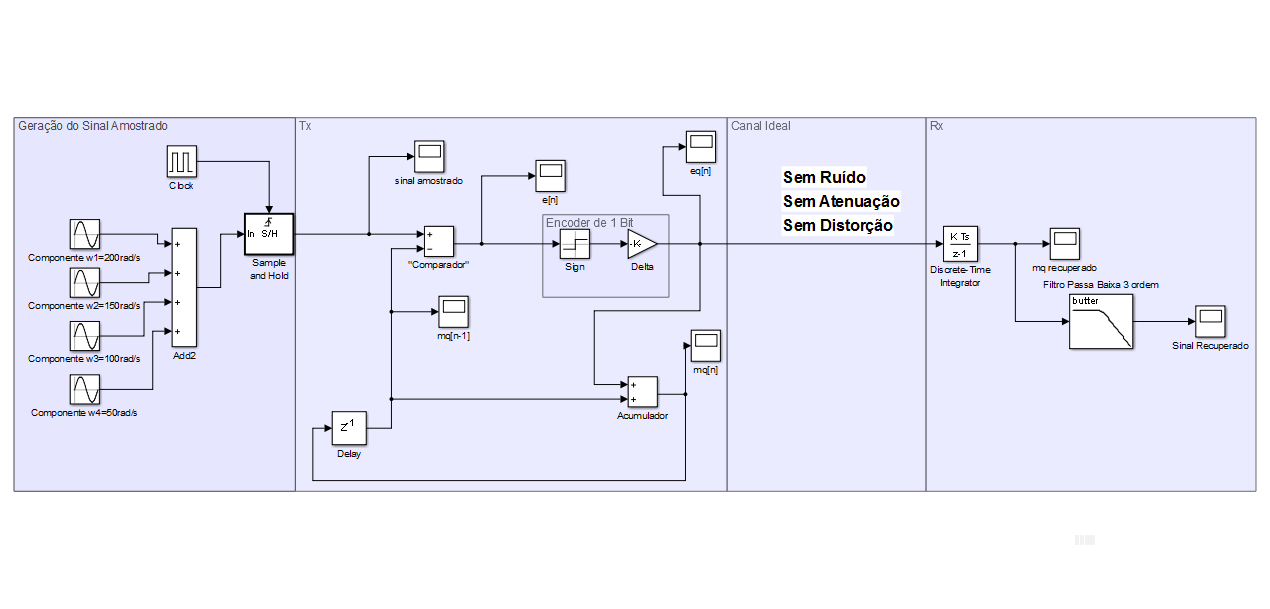
\includegraphics[width = 16 cm, height = 8 cm]{EsquemaModDelta.png}
\caption{Esquema usado para implementação da Modulação Delta}
\end{figure}

\begin{figure}
\centering
\begin{minipage}{.5\textwidth}
  \centering
  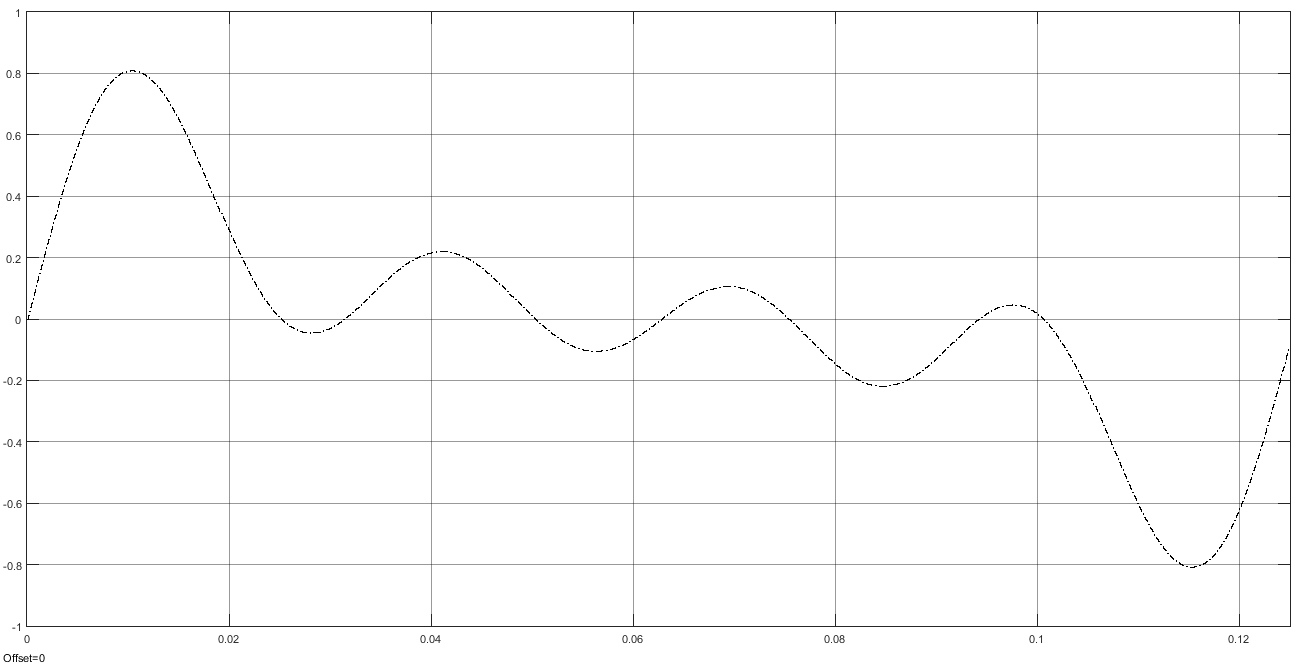
\includegraphics[width=\linewidth]{SinalAmostradoModDelta.png}
  \captionof{figure}{Sinal super amostrado}
  \label{fig:test1}
\end{minipage}%
\begin{minipage}{.5\textwidth}
  \centering
  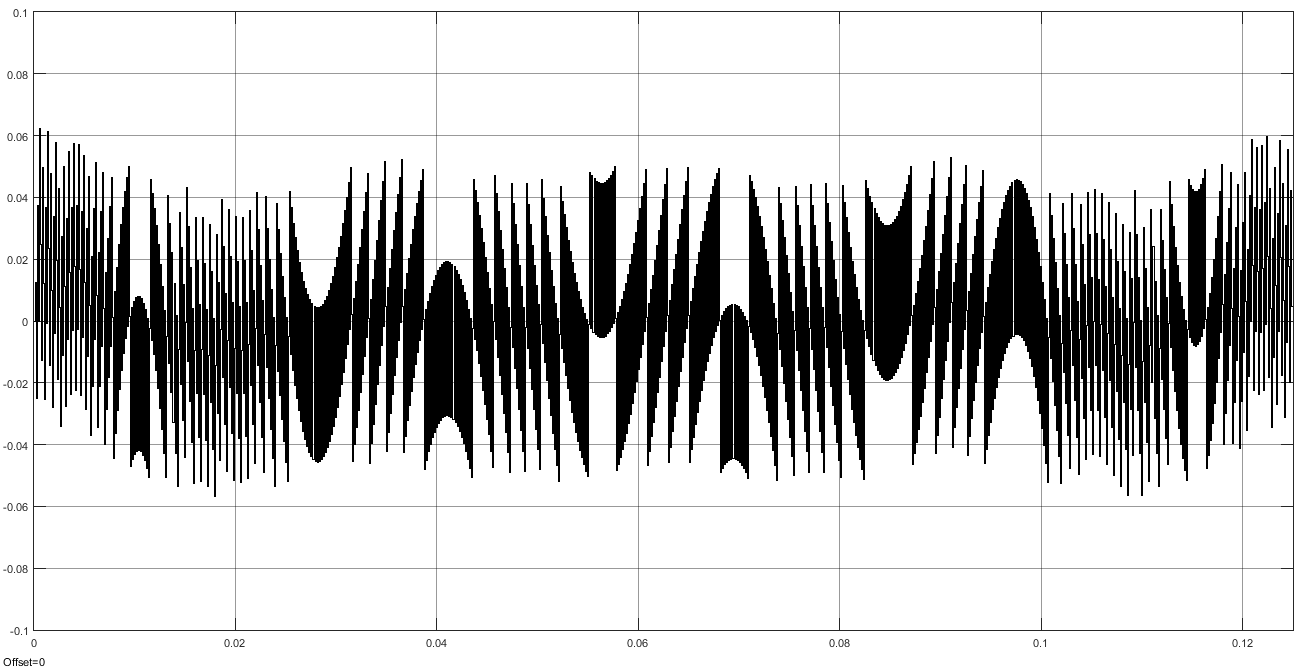
\includegraphics[width=\linewidth]{EnModDelta.png}
  \captionof{figure}{Erro e[n] entre o sinal amostrado e a aproximação do sinal $m_q[n]$}
  \label{fig:test2}
\end{minipage}
\end{figure}

\begin{figure}
\centering
\begin{minipage}{.5\textwidth}
  \centering
  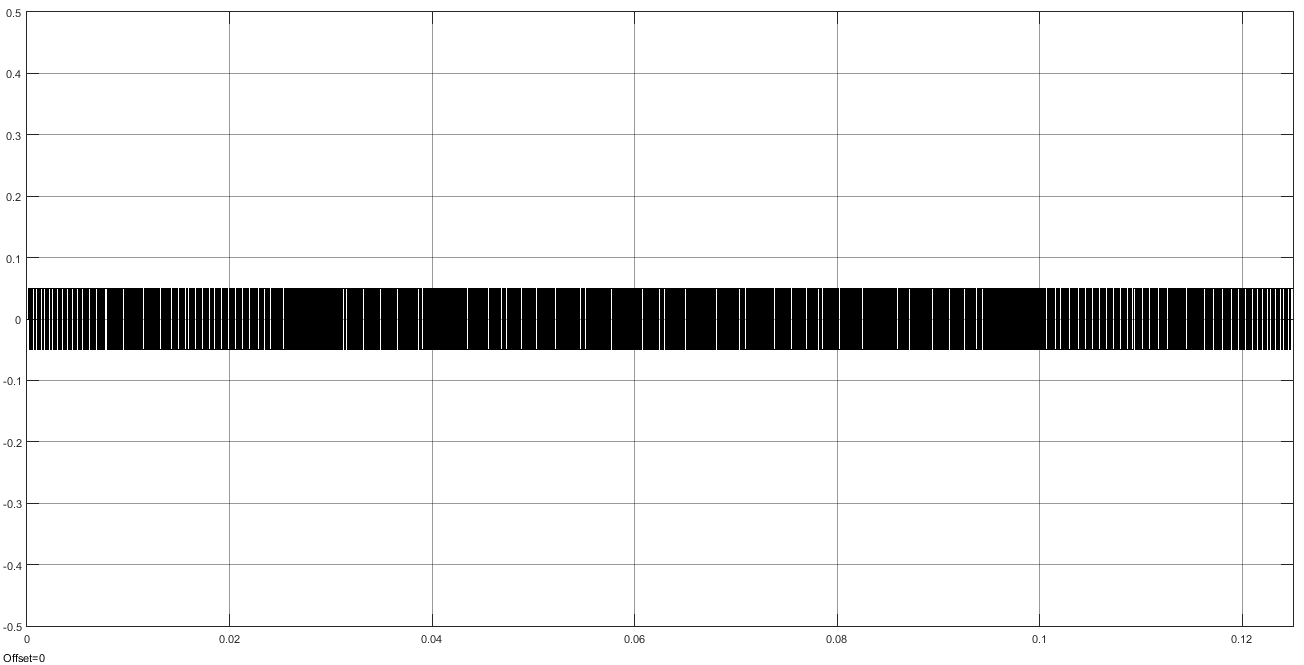
\includegraphics[width=\linewidth]{EqnModDelta.png}
  \captionof{figure}{Erro e[n] quantizado e multiplicado por $\Delta$}
  \label{fig:test3}
\end{minipage}%
\begin{minipage}{.5\textwidth}
  \centering
  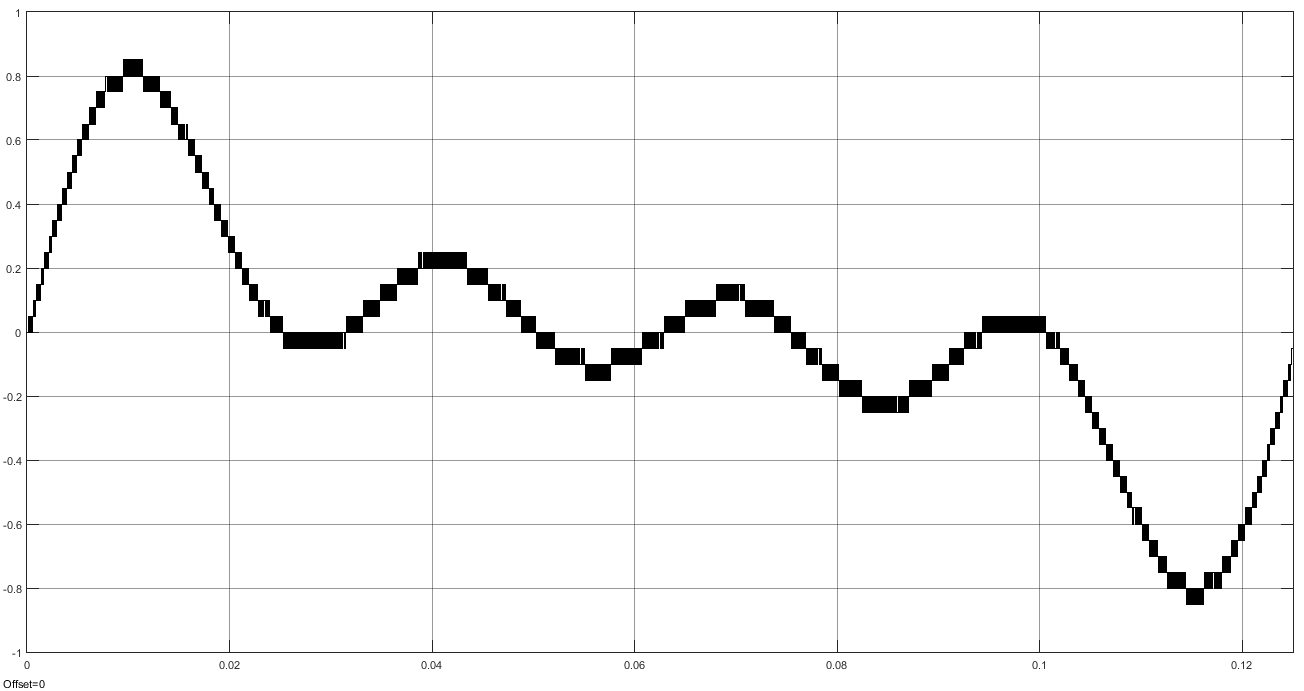
\includegraphics[width=\linewidth]{MqModDelta.png}
  \captionof{figure}{Aproximação do sinal $m_q[n]$}
  \label{fig:test4}
\end{minipage}
\end{figure}

\begin{figure}
\centering
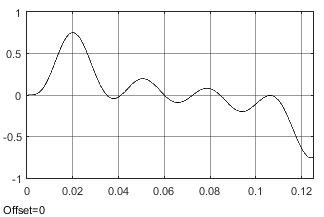
\includegraphics{SinalRecuperadoModDelta.png}
\caption{Sinal Recuperado}
\end{figure}

\section{ADPCM}
\subsection{Comentários}
O uso do PCM tradicional à uma taxa de transmissão de 64kbps para voz em muitas aplicações se torna muito custoso do ponto de vista do consumo de banda. Neste tipo de aplicação se torna necessário a codificação para atingir taxas de bit menores enquanto são mantidas a fidelidade e qualidade do áudio. Se torna necessário então o uso de um codificador de forma de onda, cuja filosofia de design tem em mente dois objetivos claros:\\

\noindent1)Remoção de redundâncias na representação do sinal.\\
2)Assinalar os bits disponíveis para as partes não redundantes do sinal de uma forma eficiente.\\

No caso do ADPCM, é possível reduzir a taxa de bits necessária para manter a mesma qualidade para 32kbps, através do uso de predição e quantização adaptativas. A modulação PCM Diferencial Adaptativa se aproveita do fato de que os sinais transmitidos geralmente tem uma característica não estacionária, isto é, a variância do sinal e autocorrelação mudam de acordo com o tempo. Este fato torna possível implementar um valor de passo para a quantização que muda de acordo com o tempo e estimativa da variância do sinal, assim como alterar os coeficientes do preditor de forma a melhor se ajustar ao sinal. 
\section{Tabela Comparativa}

\begin{table}[htbp]
  \centering
    \caption{Tabela de comparação qualitativa dos esquemas de modulação estudados}
    \begin{tabular}{ccccc}
    \textbf{Parâmetro} & \textbf{PCM} & \textbf{DPCM} & \textbf{ADPCM} & \textbf{Modulação Delta}\\
    Consumo de Banda     & Médio &  Baixo & Muito Baixo & Baixo \\
    Complexidade de Implementação     & Baixa & Média   & Alta & Muito Baixa  \\
    Ruído de Quantização     & Alto & Baixo   & Muito Baixo & Médio\\     
    \end{tabular}%

\end{table}

\section{Uso Comercial}

O ADPCM em 32kbps é aceito como um padrão internacional para transmissão de voz em conjunto com o PCM a 64kbps. Não foram encontradas aplicações comerciais da modulação Delta linear ou suas variantes na pesquisa (o que não quer dizer que não existam). 
